\section{PRIMJERI IZ INDUSTRIJE}
Implementacija autonomnih viličara više nije teorijski koncept, već standardna praksa u modernim skladištima i tvornicama. Vodeći svjetski proizvođači viličara razvili su vlastita tehnološka rješenja za automatizaciju.

\subsection{Toyota Material Handling}
Toyota, kao najveći svjetski proizvođač viličara, razvila je seriju autonomnih vozila pod nazivom \textbf{Autopilot}. Toyota Autopilot sustavi izgrađeni su na platformi njihovih standardnih ručnih viličara (poput SAE160 visokopodiznog viličara ili CDI120 horizontalnog prijenosnika paleta), što olakšava održavanje, osigurava dostupnost rezervnih dijelova i pruža visoku mehaničku pouzdanost.

% TODO: Dodane metrike i referenca za Toyotu
Primjer (ilustrativno): Toyota Autopilot flota od 50 vozila rezultirala je povećanjem \textit{throughput}-a od 20\% u distribucijskom centru \cite{toyota_case}. (TODO: provjeriti izvor).

\begin{figure}[h!]
\centering
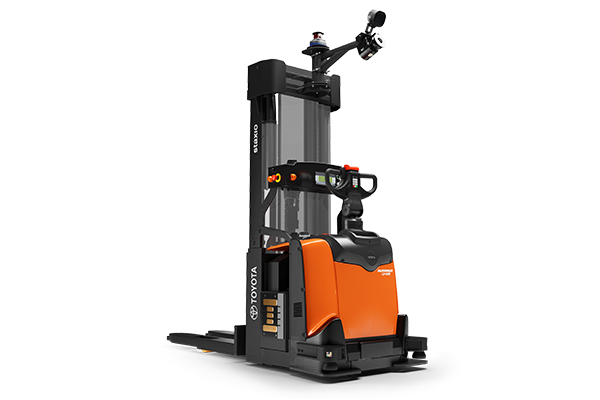
\includegraphics[width=0.7\textwidth]{slike/toyota_levio_sae160_600x400_1.png}
\caption{Toyota Autopilot viličar \cite{img_toyota}}
\label{fig:toyota}
\end{figure}

Središnji dio Toyotinog rješenja je softver \textbf{T-ONE} (\textit{Optimisation Network Enterprise}). T-ONE djeluje kao centralni sustav za upravljanje flotom (Fleet Manager) i predstavlja "mozak" skladišne automatizacije. Arhitektura T-ONE sustava temelji se na klijent-poslužitelj modelu i obavlja sljedeće kritične funkcije:
\begin{itemize}
    \item \textbf{Integracija s WMS/ERP sustavima:} T-ONE komunicira s WMS-om (npr. SAP EWM) putem web servisa (REST API ili SOAP) ili baze podataka. Kada WMS generira nalog za prijenos palete s lokacije A na lokaciju B, T-ONE zaprima taj nalog i prevodi ga u zadatak za flotu.
    \item \textbf{Dinamičko rutiranje i alokacija zadataka:} T-ONE koristi napredne algoritme za rješavanje problema usmjeravanja vozila (VRP — engl. \textit{Vehicle Routing Problem}) i pronalaženje najkraćih putova (npr. $A^*$ ili Dijkstrin algoritam na grafu skladišnih prometnica). Zadatak se dodjeljuje viličaru koji je prostorno najbliži, ima odgovarajuću razinu napunjenosti baterije i posjeduje tehničke karakteristike za taj teret.
    \item \textbf{Upravljanje prometom (Traffic Control):} Sustav sprječava zastoje (engl. \textit{deadlock} ili \textit{gridlock}) na raskrižjima skladišnih hodnika. T-ONE dinamički dodjeljuje "pravo prolaza" vozilima rezervirajući prostorne segmente (zone) na karti. Ako dva viličara idu ususret jedan drugome, sustav jednom od njih naređuje zaustavljanje ili preusmjeravanje na alternativni hodnik.
\end{itemize}

\subsection{Jungheinrich}
Njemački proizvođač Jungheinrich nudi širok spektar AGV rješenja, s posebnim naglaskom na visokoregalna skladišta i rad u uskim prolazima (VNA — engl. \textit{Very Narrow Aisle}). Primjer je viličar \textbf{EKX 516a}, automatizirani trostrani viličar za visoke regale koji omogućuje podizanje tereta na visine preko 13 metara uz milimetarsku preciznost zahvaljujući laserskom vođenju i induktivnoj navigaciji unutar regala.

% TODO: Dodane metrike i referenca za Jungheinrich
Primjer (ilustrativno): Implementacija Jungheinrich AGV rješenja u velikom proizvodnom pogonu pokazala je smanjenje operativnih grešaka za 30\% uz ROI kraći od dvije godine \cite{jungheinrich_case}. (TODO: provjeriti izvor).

\begin{figure}[h!]
\centering
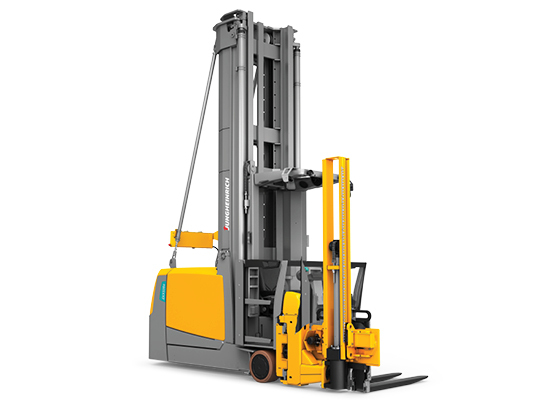
\includegraphics[width=0.7\textwidth]{slike/jungheinrich_ekx516a.jpg}
\caption{Jungheinrich EKX 516a autonomni viličar \cite{img_jungheinrich}}
\label{fig:jungheinrich}
\end{figure}

Jungheinrich se ističe integracijskim sučeljem \textbf{Logistics Interface}. To je middleware softver koji se povezuje izravno s viličarima i prevodi WMS naloge u naredbe za kretanje vozila. Glavna prednost Logistics Interface-a je plug-and-play arhitektura koja omogućuje brzu integraciju bez potrebe za kompliciranim i skupim programiranjem na strani klijentskog ERP-a.

\subsection{Gideon}
Uz globalne korporacije, važan doprinos razvoju intralogistike donose i inovativne tehnološke tvrtke poput hrvatske tvrtke \textbf{Gideon} (ranije Gideon Brothers). Gideon se na globalnom tržištu ističe razvojem naprednih sustava baziranih na 3D računalnom vidu (engl. \textit{vision-based autonomy}) koji omogućuju viličarima robusno snalaženje u vrlo dinamičnim i nepredvidivim okruženjima bez ikakve dodatne infrastrukture.

\begin{figure}[h!]
\centering
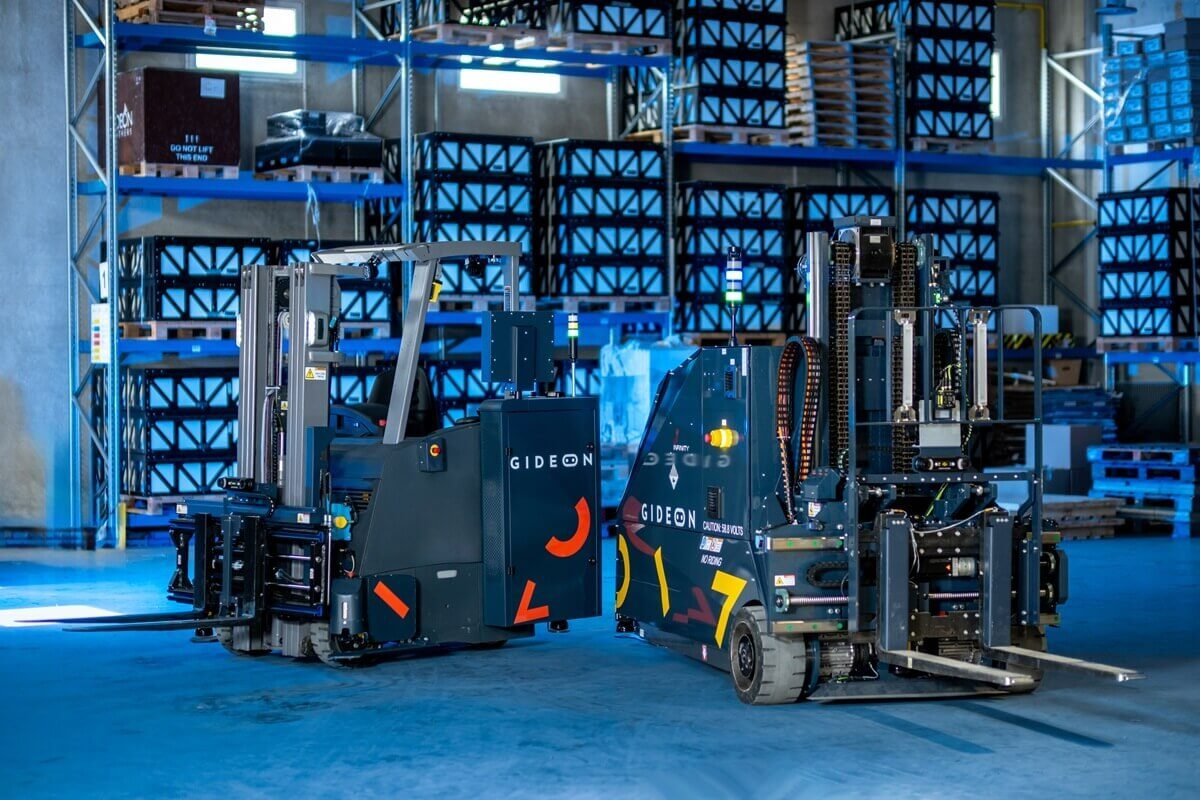
\includegraphics[width=0.7\textwidth]{slike/gideon.jpg}
\caption{Gideon autonomni viličar \cite{img_gideon}}
\label{fig:gideon}
\end{figure}

Gideon tehnologija omogućuje automatizaciju kompleksnih operacija kao što su utovar i istovar kamionskih prikolica te manipulacija teretom u proizvodnim pogonima gdje stalno dolazi do promjena rasporeda robe. Njihovi viličari projektirani su kao kolaborativni strojevi, što znači da je u potpunosti podržan hibridni rad pri kojem čovjek prema potrebi upravlja vozilom.

\subsection{Standard VDA 5050 za interoperabilnost}
Povijesno gledano, najveći problem skladišne automatizacije bio je "vendor lock-in" — situacija u kojoj je klijent morao kupovati sva vozila od istog proizvođača jer softver za upravljanje flotom tvrtke A nije mogao komunicirati s vozilima tvrtke B. Kako bi se riješio ovaj problem, Udruženje njemačke automobilske industrije (VDA) i VDMA razvili su standard **VDA 5050**.

VDA 5050 definira standardizirano komunikacijsko sučelje između upravljačkog softvera flote (Master Control) i autonomnih vozila (AGV/AMR). Komunikacija se odvija preko MQTT protokola (engl. \textit{Message Queuing Telemetry Transport}) koristeći JSON format poruka. Standard definira tri ključna kanala (teme) komunikacije:
\begin{enumerate}
    \item \textbf{Nalozi (Order):} Master Control šalje naredbe vozilu koje sadrže popis čvorova (engl. \textit{nodes}) i bridova (engl. \textit{edges}) koje vozilo mora proći, zajedno s akcijama koje treba izvršiti (npr. podigni paletu, spusti vilice).
    \item \textbf{Stanje (State):} Vozilo redovito (npr. svakih 100 ms) šalje informacije o svom trenutnom stanju, što uključuje trenutnu poziciju, brzinu, razinu baterije, aktivne greške i status izvršavanja zadanog naloga.
    \item \textbf{Vizualizacija (Visualization):} Slanje podataka o točnoj poziciji vozila visoke frekvencije radi prikaza flote u realnom vremenu na upravljačkoj ploči operatera.
\end{enumerate}
Podrškom za standard VDA 5050, moderni sustavi omogućuju stvaranje mješovitih flota u kojima, primjerice, Toyotin fleet manager koordinira rad Toyotinih autonomnih viličara i Jungheinrichovih visokoregalnih vozila, čime se drastično povećava fleksibilnost nabave i optimizacija troškova.
